\documentclass[border=5pt]{standalone}
\usepackage{pgfplots}
\usepackage{tikz}
\pgfplotsset{compat=1.18}

\begin{document}
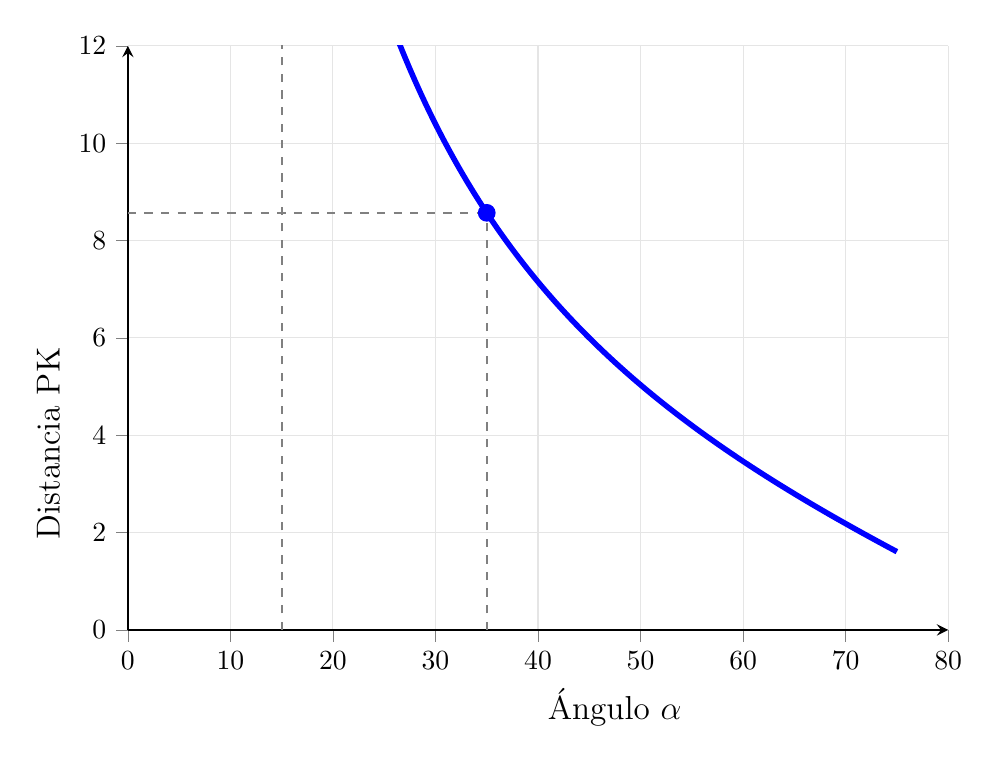
\begin{tikzpicture}
\begin{axis}[
    width=12cm,
    height=9cm,
    xlabel={Ángulo $\alpha$},
    ylabel={Distancia PK},
    xmin=0, xmax=80,
    ymin=0, ymax=12,
    grid=major,
    grid style={gray!20},
    axis lines=left,
    xlabel style={below right, font=\large},
    ylabel style={above left, font=\large},
    tick align=outside,
    xtick={0,10,20,30,40,50,60,70,80},
    ytick={0,2,4,6,8,10,12},
    samples=300,
    smooth,
    axis line style={thick},
]

% Curva hiperbólica usando cotangente
\addplot[
    blue,
    very thick,
    domain=8:75,
    samples=300,
    line width=2pt
] {6*cot(x)};

% Líneas punteadas verticales
\draw[dashed, gray, thick] (axis cs:15,0) -- (axis cs:15,{6*cot(15)});
\draw[dashed, gray, thick] (axis cs:35,0) -- (axis cs:35,{6*cot(35)});

% Líneas punteadas horizontales
\draw[dashed, gray, thick] (axis cs:0,{6*cot(15)}) -- (axis cs:15,{6*cot(15)});
\draw[dashed, gray, thick] (axis cs:0,{6*cot(35)}) -- (axis cs:35,{6*cot(35)});

% Etiquetas QP y h
\node[left, font=\Large, black] at (axis cs:-2,{6*cot(15)}) {QP};
\node[left, font=\Large, black] at (axis cs:-2,{6*cot(35)}) {h};

% Puntos en la curva
\addplot[only marks, mark=*, mark size=3pt, blue, fill=blue]
    coordinates {(15,{6*cot(15)}) (35,{6*cot(35)})};

\end{axis}
\end{tikzpicture}
\end{document}
